\documentclass{standalone} %Standalone document type to generate a high qualigy standalone pdf figure

\usepackage{graphicx}
\graphicspath{{./data/}}

\usepackage{tikz}
\usetikzlibrary{calc}
\usetikzlibrary{decorations.pathreplacing}
\usetikzlibrary{arrows.meta}

\begin{document}
    \begin{tikzpicture}
        \node[anchor=south west,inner sep=0] (image) at (0,0) {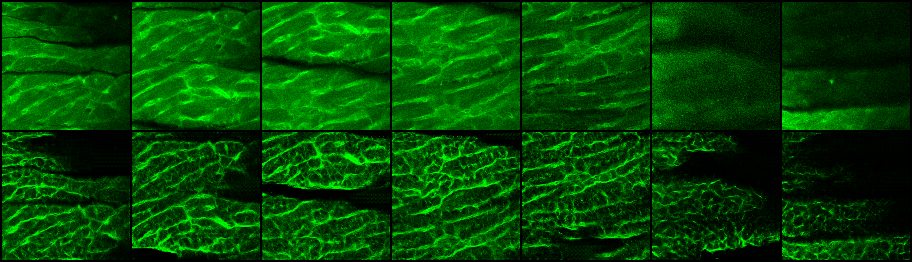
\includegraphics[width=12cm]{images/greenCells.png}};
        %%%%%%%%%%%top right box%%%%%%%%%%%%
        
        % \draw[red,very thick, rounded corners] (6.9,1.75) rectangle (12,3.45);
        % \node[red] at (9.5,3.7) {Poor SNR};
        
        
        %%%%%%%%%%bottom right %%%%%%%%%%%%%%
        
        % optional variables for numbers
        % \pgfmathsetmacro\xbrs{6.9}
        % \pgfmathsetmacro\ybrs{0}
        % \pgfmathsetmacro\xbre{12}
        % \pgfmathsetmacro\ybre{0}     
        
        %\draw [decorate,thick,decoration={brace,amplitude=10pt,mirror}] (6.9,0) -- (12,0) node [midway,below,red, yshift=-8pt,] {Hallucination};
        
        %%%%%%%%%%%%%bottom left%%%%%%%%%%%%%%%
        
        % \draw[red, very thick, rounded corners] (0,0) rectangle (5.2,1.74);
        % \node[red] at (2.5, -0.2) {Cleared}; 
        
        %%%%%%%%%%%% top left %%%%%%%%%%%%%
    
        %\draw [decorate,thick,decoration={brace,amplitude=10pt}] (0,3.5) -- (5.15,3.5) node [midway,above, yshift=10pt,green!50!black] {Higher SNR};

        %%%%%%%%%%%% Point to Salient Feature In the Image %%%%%%%%%%%%%%%%%%

        % \draw[-{Triangle[scale=0.5]}, white,line width=2pt] (1,2) -- +(60:0.5);

        % \draw[-{Triangle[scale=0.5]}, orange,line width=2pt] (6.5,1) -- +(135:0.5);
        
        %%%%%%%%%%%%%%%%%%% Comment out after annotation  %%%%%%%%%%%%%%%%
        \draw[blue] grid (12,4);
        \draw[gray, very thin, step=1mm,opacity=0.5] grid (12,4);
    \end{tikzpicture}
\end{document}